%%%%%%%%%%%%%%%%%%%%%%% file template.tex %%%%%%%%%%%%%%%%%%%%%%%%%
%
% This is a general template file for the LaTeX package SVJour3
% for Springer journals.          Springer Heidelberg 2010/09/16
%
% Copy it to a new file with a new name and use it as the basis
% for your article. Delete % signs as needed.
%
% This template includes a few options for different layouts and
% content for various journals. Please consult a previous issue of
% your journal as needed.
%
%%%%%%%%%%%%%%%%%%%%%%%%%%%%%%%%%%%%%%%%%%%%%%%%%%%%%%%%%%%%%%%%%%%
%
% First comes an example EPS file -- just ignore it and
% proceed on the \documentclass line
% your LaTeX will extract the file if required
\begin{filecontents*}{example.eps}
%!PS-Adobe-3.0 EPSF-3.0
%%BoundingBox: 19 19 221 221
%%CreationDate: Mon Sep 29 1997
%%Creator: programmed by hand (JK)
%%EndComments
gsave
newpath
  20 20 moveto
  20 220 lineto
  220 220 lineto
  220 20 lineto
closepath
2 setlinewidth
gsave
  .4 setgray fill
grestore
stroke
grestore
\end{filecontents*}
%
\RequirePackage{fix-cm}
%
%\documentclass{svjour3}                     % onecolumn (standard format)
%\documentclass[smallcondensed]{svjour3}     % onecolumn (ditto)
\documentclass[smallextended,final]{svjour3}       % onecolumn (second format)
%\documentclass[twocolumn]{svjour3}          % twocolumn
%
\smartqed  % flush right qed marks, e.g. at end of proof
%
\usepackage[dvipdfmx]{graphicx}
\usepackage{amsmath}
\usepackage{amsfonts}
\usepackage{comment}
\usepackage{color}
\newcommand{\postpone}{\textcolor{red}{[MEMO]:あとでかく}}
%
% \usepackage{mathptmx}      % use Times fonts if available on your TeX system
%
% insert here the call for the packages your document requires
%\usepackage{latexsym}
% etc.
%
% please place your own definitions here and don't use \def but
% \newcommand{}{}
%
\newcommand{\rank}{\mathrm{rank} \ }
\newcommand{\trank}{\mathrm{term}\mbox{-}\mathrm{rank} \ }
% Insert the name of "your journal" with
% \journalname{myjournal}
%
\begin{document}

\title{ %Computing All Maximum Degrees of Minors \\ in Rational Matrices via Combinatorial Relaxation\\
Combinatorial Relaxation Algorithm \\ for Entire Sequence of Maximum Degree of Minors
%\thanks{Grants or other notes
%about the article that should go on the front page should be
%placed here. General acknowledgments should be placed at the end of the article.}
}
%\subtitle{Do you have a subtitle?\\ If so, write it here}

%\titlerunning{Short form of title}        % if too long for running head

\author{Kazuo Murota \and Shun Sato %etc.
}

%\authorrunning{Short form of author list} % if too long for running head

\institute{K. Murota \at
              Department of Mathematical Informatics, Graduate School of Information Science and Technology, University of Tokyo, Tokyo 113-8656, Japan \\
              %Tel.: +123-45-678910\\
              %Fax: +123-45-678910\\
              \email{murota@mist.i.u-tokyo.ac.jp}    %  \\
%             \emph{Present address:} of F. Author  %  if needed
           \and
           S. Sato \at
              Department of Mathematical Informatics, Graduate School of Information Science and Technology, University of Tokyo, Tokyo 113-8656, Japan. %\email{shun_sato@mist.i.u-tokyo.ac.jp}
}

\date{Received: date / Accepted: date}
% The correct dates will be entered by the editor


\maketitle

\begin{abstract}
%Maximum degree of minors in rational matrices is useful for finding Smith--McMillan form at infinity. 
This paper presents an efficient algorithm for computing the entire sequence of maximum degree of minors, 
whereas the previous one find them of a specified order $k$. 
The efficiency derives from good properties of valuated bimatroids such as concavity. 

The present algorithm adopts “combinatorial relaxation” 
which is a general framework with practical efficiency and accuracy. 
Combinatorial relaxation type algorithm first solves the relaxation problem, 
weighted bipartite matching problem in our case, to obtain an estimate on optimal value. 
Then, it checks the estimate is correct or not. 
If it is incorrect, 
the algorithm modifies the problem to improve the estimate without affecting the optimal value.

\keywords{Combinatorial relaxation \and Degree of minor \and Valuated bimatroid}
% \PACS{PACS code1 \and PACS code2 \and more}
% \subclass{MSC code1 \and MSC code2 \and more}
\end{abstract}

\section{Introduction}
\label{intro}

Finding the maximum degree of minors is fundamental problem in engineering. 
Smith--McMillan form at infinity and Kronecker form is important application of maximum degree of minors.
Smith--McMillan form at infinity is a normal form of rational matrices 
and important in the control theory(Commault--Dion\cite{SMF}).
Kronecker form is a normal form of matrix pencils and it can be used to analyze DAEs(Gear\cite{DAE}).
They needs the entire sequence of maximum degree of minors. 
Therefore, we propose the efficient combinatorial relaxation type algorithm 
for finding the entire sequence of maximum degree of minors 
whereas previous one (\cite{PDCRA,PCRA}) find it of specified order $k$. 

Murota\cite{PCRA,DCRA} shows that 
“combinatorial relaxation” can be used to find the maximum degree of minors in rational matrices. 
Combinatorial relaxation algorithm is the framework due to Murota\cite{CRA}. 
Generally, combinatorial relaxation type algorithm constructed as follows:
\begin{description}
\item{{\bf Step 1:}} Consider the combinatorial relaxation (e.g. matching on bipartite graph) and solve it.
\item{{\bf Step 2:}} Test wether combinatorial relaxation is equal to optimal solution or not without knowing optimal solution itself. 
\item{{\bf Step 3:}} In the case of incorrectness, modify the problem and go back to Step 1.
\end{description}

Combinatorial relaxation algorithm has practical efficency like “graph theoretic approach(Lin\cite{SC})” 
and accuracy like numerical method.

This paper is constructed as follows:
First, the preliminaries such as the definition of maximum degree of minors in section \ref{pre}. 
Next, we propose the combinatorial relaxation algorithm for the entire sequence of maximum degree of minors in section \ref{cra}.
Then, we analyze time complexity of the proposed algorithm theoretically in section \ref{ca} and 
conclude this paper in section \ref{conc}.



\section{Preliminaries}
\label{pre}
\subsection{Rational Matrices and Maximum Degree of Minors}
\label{rfm}
Let $ A (x) $ be a rational matrix over a field $F$, 
i.e., for all row $ i $ and column $j$, $ A_{ij} (x) $ is rational function in $x$ over $F$.
Typically, $ F $ is the real number field $ \mathbb{R} $ or 
the rational number field $\mathbb{Q}$.
We define the degree of rational function $ f (x) = p(x) / q(x)$ by $ \deg f = \deg p - \deg q $.
If $ f(x) = 0 $, we denote $ \deg f = - \infty $ by convention. 
The maximum degree of minors of order $k$ is defined as follows:
\begin{equation}
\delta_k (A) := \max \left\{ \deg  \det A[I,J] \mid I \subseteq \mathrm{Row} (A), \ J \subseteq \mathrm{Col} (A), \  |I| = |J| = k \right\}.
\end{equation}
$\delta_0 (A) $ is defined as $ \delta_0 (A) = 0 $. 
$ A[I,J] $ denotes the submatrix of $A(x) $ with row-set $I$ and column-set $J$.

\subsection{Smith--McMillan Form at Infinity}
\label{smf}
We call a rational function $ f(x) $ proper if $ \deg f \le 0 $. 
A rational matrix is said to be a proper rational matrix if its all entries are proper. 
We call a square proper rational matrix $U(x)$ biproper 
if it is invertible and $ U^{-1} (x) $ is proper.
For a proper rational matrix $ U(x) $, 
following two conditions are equivalent(see e.g. \cite{MMSA}):
\begin{itemize}
\item $U(x)$ is a biproper rational matrix;
\item $ \det U (x) $ is a nonzero constant.
\end{itemize}

Any rational matrix can be brought into the Smith--McMillan form at infinity(Verghese--Kailath\cite{RMS}).
\begin{proposition}
Let $ A(x) $ be a rational matrix and denote its rank by $r$. 
There exist biproper rational matrices $U(x) $ and $ V(x) $ such that 
\[ U(x) A(x) V(x) = \begin{pmatrix} \Gamma (x) & O \\ O & O \\ \end{pmatrix}, \]
where 
\[ \Gamma (x) = \mathrm{diag} ( x^{t_1},\dots, x^{t_r}), \]
and $ t_k \ ( k = 1, \dots ,r) $ are nonincreasing integers, 
i.e., $ t_1 \ge \dots \ge t_r $.
Moreover, $ t_k $ satisfies following equation:
\[ t_k = \delta_k (A) - \delta_{k-1} (A) \quad ( k = 1 ,\dots ,r). \]
\end{proposition}

The transformation such as: $ U(x) A(x) V(x) $ is called biproper equivalence transformations 
if $U(x)$ and $V(x)$ are biproper rational matrices.
It is important fact that $ \delta_k (A) $'s are invariant 
under the biproper equivalence transformations. 

\subsection{Combinatorial Relaxation}
\label{CR}

Let $ A(x) $ be a rational matrix with row set $R$ and the column set $C$. 
We define $ G(A) = ( R \cup C , E(A) , c) $ be a bipartite graph assciated with $ A(x) $ 
where arc set $ E(A) $ and weight $ c : E(A) \to \mathbb{Z}$ is defined as follows:
\begin{align}
E(A) &= \left\{ (i,j) \mid i \in R , \ j \in C , \ A_{ij} (x) \neq 0 \right\},\\
c(i,j) &= \deg A_{ij} \quad ( (i,j) \in E(A) ).
\end{align}

We define $ \hat{\delta}_k (A) $ be a maximum weight matching of size $k$ in $G(A) $, i.e.,
\begin{equation}
\hat{\delta}_k (A) = \max \left\{ c(M) \mid M:\mathrm{a \ matching \  in \ } G(A) ,\ |M| = k \right\}
\end{equation}
where $ c(M) = \sum_{ (i,j) \in M } c (i,j) $. 
If there are no matching of size $k$ in $G(A)$, we denote $ \hat{\delta}_k (A) = - \infty$.
$ \hat{\delta}_k (A) $ can be computed efficiently by Hungarian method\cite{HM}.

$ \hat{\delta}_k (A) $ plays the role as a combinatorial relaxation of $ \delta_k (A) $ 
because following inequality holds(\cite[Theorem 3]{PCRA}):
\begin{equation}
\delta_k (A) \le \hat{\delta}_k (A). \label{ineqd}
\end{equation}

The duality of linear programming problem plays an essential role 
for testing whether $ \delta_k (A) = \hat{\delta}_k (A) $ or $ \delta_k (A) < \hat{\delta}_k (A)$. 
The primal-dual pair of linear programming problems are defined as follows:
\begin{align}
\mathrm{PLP(A,k): \  maximize} \quad  & \sum_{e \in E} c_e \xi_e, \notag \\
\mathrm{subject \  to}      \quad     & \sum_{ \partial e \ni i } \xi_e \le 1 \quad ( i \in V ), \label{defplp} \\
                                      & \sum_{ e \in E } \xi_e = k, \notag \\
                                      & \xi_e \ge 0 \quad ( e \in E ); \notag \\
\mathrm{DLP(A,k): \  minimize} \quad  & \sum_{i \in R} p_i + \sum_{j \in C} q_j + k t \quad ( \equiv \pi (p,q,t) ), \notag \\
\mathrm{subject \  to} \quad   & p_i + q_j + t \ge c_{ij} \quad ((i,j) \in E), \label{defdlp} \\
                               & p_i \ge 0 \quad ( i \in R ), \notag\\
                               & q_j \ge 0 \quad ( j \in C ). \notag
\end{align}
PLP($A,k$) and DLP($A,k$) has an integral optimal solution, 
and their optimal values are equall to $ \hat{\delta}_k (A) $.

We define active rows $ I^{\ast} \subseteq R $ and columns $ J^{\ast} \subseteq C $ as follows:
\begin{align}
I^{\ast} &= I^{\ast} (p) = \left\{ i \in R \mid p_i > 0 \right\}, \label{eqdefar}\\
J^{\ast} &= J^{\ast} (q) = \left\{ j \in C \mid q_j > 0 \right\}. \label{eqdefac}
\end{align}
Moreover, we define tight coefficient matrix $ A^{\ast} $ as follows:
\begin{equation}
A^{\ast}_{ij} = \lim_{ x \to \infty } x^{ -p_i - q_j - t } A_{ij} (x). \label{eqdefaa}
\end{equation}

Proposition \ref{prop4r} enables us to test whether $ \delta_k (A) = \hat{ \delta}_k (A) $ or not 
without knowing $ \delta_k (A) $.

\begin{proposition}[\cite{PCRA} Theorem 4]
Let $ (p,q,t) $ be an optimal dual solution, 
$I^{\ast}$ and $ J^{\ast} $ be the active rows and columns defined by (\ref{eqdefar}) and (\ref{eqdefac}), 
and $ A^{\ast} $ be the tight coefficient matrix defined by (\ref{eqdefaa}). 
Then $ \delta_k (A) = \hat{\delta}_k (A) $ if and only if the following four conditions are satisfied:
\begin{description}
\item[{\em (r1)}] $ \rank A^{\ast} [ R ,C ] \ge k $,
\item[{\em (r2)}] $ \rank A^{\ast} [I^{\ast},C] = | I^{\ast} | $,
\item[{\em (r3)}] $ \rank A^{\ast} [ R , J^{\ast} ] = | J^{\ast} | $,
\item[{\em (r4)}] $ \rank A^{\ast} [ I^{\ast},J^{\ast} ] \ge | I^{\ast} | + |J^{\ast} | - k $.
\end{description}
\label{prop4r}
\end{proposition}

\subsection{Valuated Bimatroids}
\label{vb}
The concept of a valuated bimatroid is defined by Murota\cite{VB} 
as a variant of a valuated matroid (Dress--Wenzel\cite{VM1,VM2}). 
And the valuation $w$ of valuated bimatroids represents the abstract property of degree of minors in rational matrices.

\begin{definition}[Valuated Bimatroid]
Let $ R $ and $ C $ be disjoint finite sets. 
And let $ w : 2^R \times 2^C \to \mathbb{R} \cup \{ - \infty \} $ be a map. 
We define $ ( R, C, w ) $ to be a valuated bimatroid 
if and only if $ w $ satisfies $ w( \emptyset , \emptyset) \neq - \infty $, 
$ w (I,J) = - \infty $ for $( I,J) \notin S $ where
\[ S = \{ (I,J) \mid |I| = |J|, \  I \subseteq R , \ J \subseteq C \}, \]
and the exchange properties (E1) and (E2) below 
for any $ (I,J) \in S $ and $ ( I' ,J' ) \in S $:
\begin{description}
\item[(E1)] For any $ i' \in I' \setminus I$, (a1) or (b1) holds:
\begin{description}
\item[(a1)] $ \exists j' \in J' \setminus J :$ $ w(I,J) + w(I',J') \le w(I+ i', J+ j') + w ( I' - i' , J' - j') $,
\item[(b1)] $ \exists i \in I \setminus I' :$ $ w(I,J) + w(I',J') \le w(I - i + i', J) + w ( I' - i' + i , J' ) $.
\end{description} 
\item[(E2)] For any $ j \in J \setminus J' $, (a2) or (b2) holds:
\begin{description}
\item[(a2)] $ \exists i \in I \setminus I' :$ $ w(I,J) + w(I',J') \le w(I - i , J - j) + w ( I' + i , J' + j ) $,
\item[(b2)] $ \exists j' \in J' \setminus J :$ $ w(I,J) + w(I',J') \le w(I , J - j + j') + w ( I' , J' - j' + j) $.
\end{description} 
\end{description}
\end{definition}

We define 
$ S_k \subseteq S ,$ $ \delta_k \in \mathbb{Z}, $ $ M_k \subseteq S_k \times S_k $ 
as follows:
\begin{align*}
S_k &= \{ (I,J) \mid |I| = |J| = k, \ I \subseteq R , \ J \subseteq C \},\\
\delta_k &= \max \{ w (I,J) \mid (I,J) \in S_k \},\\
M_k &= \{ (I,J) \in S_k \mid w(I,J) = \delta_k \}.
\end{align*} 

\begin{proposition}[Murota\cite{VB} Theorem 1]
The following inequality holds:
\begin{equation}
\delta_{k-1} + \delta_{k+1} \le 2 \delta_k, \quad ( k = 1 ,2, \dots , r-1) \label{eqcon}
\end{equation}
\label{propc}
\end{proposition}

Since $ w(I,J) := \deg \det A[I,J] $ and $ w (I,J) := \max \{ c(M) \mid M \subseteq E(A) ,$ 
$\partial M = I \cup J \}$ define valuated bimatroids $ (R,C,w) $, 
Proposition \ref{propc} means that $ \{ \delta_k (A) \}_{k=0}^r $ 
and $ \{ \hat{\delta}_k (A) \}_{k=0}^r $ have concavity. 

\begin{proposition}[Murota\cite{VB} Theorem 2]
For any $(I_k ,J_k) \in M_k $ with $ k = 1, \dots ,r-1 $, 
there exists $(I_l,J_l) \in M_l \ ( 0 \le l \le r , l \neq k ) $ such that 
$ ( \emptyset = ) I_0 \subseteq I_1 \subseteq \dots \subseteq I_{k-1} \subseteq I_k \subseteq I_{k+1} \subseteq \dots \subseteq I_r $ 
and 
$ ( \emptyset = ) J_0 \subseteq J_1 \subseteq \dots \subseteq J_{k-1} \subseteq J_k \subseteq J_{k+1} \subseteq \dots \subseteq J_r $.
\label{propn}
\end{proposition}









% % % % % % % % % % % % % % % % % % % % %  Combinatorial Relaxation Algorithm % % % % % % % % % %


\section{Combinatorial Relaxation Algorithm}
\label{cra}
In this section, 
we propose a combinatorial relaxation algorithm 
for computing the entire sequence of maximum degree of minors $\{ \delta_k (A) \}_{k=1}^r$ 
where $ A(x) $ be a Laurent polynomial matrix and $ r = \rank A(x) $.
The proposed algorithm has 4 properties as follows:
\begin{itemize}
\item In the end of the algorithm, $ \delta_k (A) = \hat{\delta}_k (A) $ is satisfied for all $k = 1 , \dots ,r $;
\item The number of the constant matrix which need to compute its rank for testing the tightness is only one, whereas previous one need 4 matrices;
\item In the step of matrix modification, the size of matrix multiplication is reduced;
\item During $ \delta_k (A) $ is increasing(decreasing) at same rate, we can skip the computation.
\end{itemize}

The outline of the algorithm is summarized as follows.

\vspace{0.5zw}

\noindent
{\bf Outline of Algorithm for Computing} $ \{ \delta_k (A) \}_{k=1}^r $\\
\begin{tabular}{ll}
{\bf Step 0:} & Compute $ \delta_1 (A) $ and set $k:=1$.\\
{\bf Step 1:} & Find an optimal solution $(p,q,t)$ of DLP($A,k$).\\
{\bf Step 2:} & Test whether $ \delta_{k+1} (A) = \hat{\delta}_{k+1} (A) $ or not by using $(p,q,t)$. \\
              & If equality holds, go to Step 4.\\
{\bf Step 3:} & Modify $ A(x) $ to $ A' (x) $, and go back to Step 1. \\
{\bf Step 4:} & Output optimal values, update $k$ and go back to Step 1. \\
\end{tabular}
\vspace{0.5zw}

We detail the algorithm description in \ref{description}.

For initialization, we find $ (i,j) \in R \times C $ such that a maximizer of $ \deg A_{ij} $. 
Since $ \delta_1 (A) = \hat{ \delta}_1 (A) = \deg A_{ij} $ holds, 
we define $ I^{\ast}_1 = \{ i \}, $ $J^{\ast}_1 =\{ j \},$ $M_1 = \{ (i,j) \} $. 


\subsection{Construction of an Optimal Dual Solution}
\label{dual}
When we execute Step 1, following conditions hold:
\begin{itemize}
\item $ \delta_l (A) = \hat{ \delta }_l (A) \quad ( l = 1,2,\dots ,k)$;
\item $ \deg \det A [I^{\ast}_k , J^{\ast}_k] = \sum_{ (i,j) \in M_k } \deg A_{ij} = \delta_k (A)$;
\item $ I^{\ast}_k = \partial^+ M_k ,$ $ J^{\ast}_k = \partial^- M_k $.
\end{itemize}
In fact, we don't need to store $ I^{\ast}_k $ and $ J^{\ast}_k $ 
because they can be easily constructed from $M_k$.
But they are helpful for describing and comprehending the proposed algorithm.

In this step, we introduce the method to construct an optimal dual solution.
As stated in Iwata--Takamatsu\cite{MP}, 
we can obtain it by solving shortest path problem on the auxiliary graph. 
Consider an auxiliary graph $ G_{M_k} = (V,E,\gamma) $ associated with $ M_k $ where 
\begin{align*}
V &= R \cup C \cup \{ u^+ \} \cup \{ u^- \},\\
E &= E(A) \cup M^{\circ} \cup W^{+} \cup W^{-}.
\end{align*}
Here, $ u^{+} $ and $ u^{-} $ are new vertices and 
\begin{align*}
E(A) &= \left\{ (i,j) \mid i \in R , \ j \in C , \ A_{ij} (x) \neq 0 \right\},\\
M^{\circ} &= \left\{ (j,i) \mid (i,j) \in M_k \right\},\\
W^{+} &= \left\{ ( u^{+} , i) \mid i \in R \setminus I^{\ast}_k \right\},\\
W^{-} &= \left\{ (j,u^{-}) \mid j \in C \setminus J^{\ast}_k  \right\} \cup \{ (u^-,j) \mid j \in C \}.
\end{align*}
We define the arc length $ \gamma : E \to \mathbb{Z} $ by
\[ \gamma (i,j) = \begin{cases} - \deg A_{ij} \quad & \left( (i,j) \in E(A) \right),\\
                              \deg A_{ji}   \quad & \left( (i,j) \in M^{\circ} \right),\\
                              0                   & \left( (i,j) \in W^{+} \cup W^{-} \right). \end{cases} \]
Let $ \varphi (i) $ be the length of a shortest path from $ u^+ $ to $ i \in V $ 
with arc length $ \gamma $ in $ G_{M_k} $. 
If there is no path from $ u^+ $ to $ i \in V $, we put $ \varphi (i) = + \infty $.
We define $ (p,q,t) $ as follows:
\begin{align}
p_i &= \varphi (i) & ( i \in R ), \notag \\
q_j &= \varphi(u^-) - \varphi (j) & ( j \in C ), \label{eqdefpq}\\
t   &= - \varphi(u^-). \notag
\end{align}

If there is a path from $ u^+ $ to $ u^- $, $ (p,q,t) $ is an optimal dual solution of DLP$ (A,k) $ 
as Lemma \ref{lemoptdual}. 
In other case, i.e., there is no path from $ u^+ $ to $ u^- $, 
$ k = \rank A(x) $ holds ($ k = \trank A (x) \ge \rank A(x) $).

Lemma \ref{lemoptdual} is slightly different version of \cite[Lemma 3]{MP}.

\begin{lemma}
Let $ M_k $ be a maximum weight matching with $ |M_k| = k $ in $ G(A) $. 
$ ( p,q,t) $ defined as the equation (\ref{eqdefpq}) 
with $ G_{M_k} $ is an optimal dual solution of $ \mathrm{DLP} (A,k) $. 
Furthermore, if a weight function is integer valued, 
then $ (p,q) $ is an integral solution.
\label{lemoptdual}
\end{lemma}

In this step, we can adopt “reweighting” like Johnson's algorithm (see e.g. \cite{AI}) 
for all-pairs shortest path. 
And we can use the newest optimal dual variable for reweighting \cite{TI,TNP} in this case.

\subsection{Test for Tightness}
\label{test}

Testing for tightness, 
we adopt Theorem \ref{thmtest} instead of Proposition \ref{prop4r}.
Following lemma is essential for Theorem \ref{thmtest} and other theorems.

\begin{lemma}
Under the condition of Lemma \ref{lemoptdual}, 
$(p,q,t)$ is an optimal dual solution of $ \mathrm{DLP} (A,k+1) $.
\label{lemoptdualnext}
\end{lemma}

\begin{proof}
Since $ (p,q,t) $ is obviously a feasible solution of DLP$(A,k+1)$, we prove only optimality.

The objective function of DLP($A,k+1$) is expressed as:
\[ \pi_{k+1} (p,q,t) = \sum_{ i \in R } p_i + \sum_{ j \in C} q_j + (k+1) t = \pi_k (p,q,t) + t. \]
On the other hand, since dual variable $t = - \varphi (u^-) $ is defined as the maximum length of augmenting path, 
the opimal value of DLP($A,k+1$) is $t$ more than the optimal value of DLP($A,k$). 
Therefore, $(p,q,t) $ is one of the optimal dual solution of DLP($A,k+1$).  \qed
\end{proof}

\begin{theorem}
Suppose that $ \delta_k (A) = \hat{\delta}_k (A) $ holds 
and $ M_k $ is a maximum weight matching of size $k$ in $G(A)$.
Let $(p,q,t)$ be a dual variable defined as (\ref{eqdefpq}) from $M_k$ 
and $ A^{\ast} $ be a tight coefficient matrix defined as (\ref{eqdefaa}). 
Then, following 2 conditions are equivallent:
\begin{itemize}
\item $\delta_{k+1} (A) = \hat{\delta}_{k+1} (A) = \delta_k (A) + t$.
\item $\rank A^{\ast} \ge k + 1 $.
\end{itemize}
\label{thmtest}
\end{theorem}

\begin{proof}
Since $ \delta_k (A) = \hat{\delta}_{k} (A) $ holds, 
following 4 conditions are satisfied by Proposition \ref{prop4r}:
\begin{description}
\item[(r1)] $ \rank A^{\ast} [R,C] \ge k $,
\item[(r2)] $ \rank A^{\ast} [I^{\ast},C] = | I^{\ast} | $,
\item[(r3)] $ \rank A^{\ast} [R,J^{\ast}] = | J^{\ast} | $,
\item[(r4)] $ \rank A^{\ast} [I^{\ast} ,J^{\ast} ] \ge |I^{\ast} | + | J^{\ast} | - k  $.
\end{description}

On the other hand, by Lemma \ref{lemoptdualnext} and Proposition \ref{prop4r}, 
$ \delta_{k+1} (A) = \hat{\delta}_{k+1} (A) $ holds 
if and only if following 4 conditions are all satisfied:
\begin{description}
\item[(r1)'] $ \rank A^{\ast} [R,C] \ge k+1 $,
\item[(r2)'] $ \rank A^{\ast} [I^{\ast},C] = | I^{\ast} | $,
\item[(r3)'] $ \rank A^{\ast} [R,J^{\ast}] = | J^{\ast} | $,
\item[(r4)'] $ \rank A^{\ast} [I^{\ast} ,J^{\ast} ] \ge |I^{\ast} | + | J^{\ast} | - k -1 $.
\end{description}
Clearly, (r2)', (r3)' and (r4)' immediately derives from (r2), (r3) and (r4).
Therefore, $ \delta_{k+1} (A) = \hat{\delta}_{k+1} (A) \iff \rank A^{\ast} \ge k + 1 $. \qed
\end{proof}

Since Theorem \ref{thmtest} holds, 
we can test whether $ \delta_{k+1} (A) = \hat{\delta}_{k+1} (A) $ or not 
by calculation of $ \rank A^{\ast}$. 



\subsection{Matrix Modification}
\label{mod}

Theorem \ref{thmtest} enable us to consider only the case $ \rank A^{\ast} = k $ 
whereas existing algorithms cope with 4 cases.
When we implement Step 3, following conditions are satisfied:
\begin{enumerate}
\item $ \rank A^{\ast} = k $,
\item $ \rank A^{\ast} [I^{\ast}_l, J^{\ast}_l] = l \quad ( l = 1 ,2 , \dots ,k)$.
\end{enumerate}
Therefore, there exists $ m \times m $ constant matrix $ U $ such that
\begin{description}
\item[(U1)] $ U[I^{\ast}_k,I^{\ast}_k]$ and $ U [R \setminus I^{\ast}_k, R \setminus I^{\ast}_k]$ are identity matrices,
\item[(U2)] $ U[I^{\ast}_k,R \setminus I^{\ast}_k] = O $,
\item[(U3)] $ \trank U A^{\ast} = k$.
\end{description}
Namely, we can interpret (U1), (U2) and (U3) as
\[ U A^{\ast} = \left( \begin{array}{cc} I & O \\ \tilde{U} & I \\ \end{array} \right) A^{\ast} = \left( \begin{array}{c} A^{\ast} [I^{\ast}_k,C] \\ O \end{array} \right) \]
by appropriate permutation. 
Where $I$ denote an identity matrix of suitable order 
and $ \tilde{U} = U[R \setminus I^{\ast}_k,I^{\ast}_k] $ is an constant matrix. 

We can modify the matrix $ A(x) $ by the constant matrix $U$ 
such that (U1), (U2) and (U3) are satisfied.
Let $ A'(x) $ be the modified matrix, then we define 
\begin{equation}
A'(x) = \mathrm{diag} (x;p) \cdot U \cdot \mathrm{diag} (x;-p) \cdot A(x). \label{eqmod}
\end{equation}
The right side of the equation (\ref{eqmod}) can be computed 
by partial matrix multiplication as follows:
\begin{align}
A'(x)
&= \mathrm{diag} (x;p) \cdot \left( \begin{array}{cc} I & O \\ \tilde{U} & I \end{array} \right) \cdot  \mathrm{diag} (x;-p) \cdot A(x) \\
&= \left( \begin{array}{cc} I & O \\ \tilde{U} \cdot \mathrm{diag} (x;-p^{\ast}_k) & I \end{array} \right)  \left( \begin{array}{c} A[I^{\ast}_k ,C] (x) \\ A[ R \setminus I^{\ast}_k ,C] (x) \end{array} \right)
\end{align}
where $p^{\ast}_k = ( p_i \mid i \in I^{\ast}_k)$. Therefore, 
\begin{align}
A'[I^{\ast}_k,C] &= A[I^{\ast}_k ,C] (x), \label{eqinv}\\
A'[R \setminus I^{\ast}_k ,C] &= \tilde{U} \cdot \mathrm{diag} (x:-p^{\ast}_k) \cdot A[ I^{\ast}_k,C] (x) + A[R \setminus I^{\ast}_k ,C ] .
\end{align}

We claim that this modification makes sense as stated in Theorem \ref{thmmod}.

\begin{theorem}
A matrix $ A'(x) $ defined as (\ref{eqmod}) has following 4 properties:
\begin{enumerate}
\item $ \delta_l (A') = \delta_l (A) \quad ( l = 1 ,\dots,r) $;
\item $ \deg \det A' [ I^{\ast}_k,J^{\ast}_k] = \delta_k (A')$;
\item $ \hat{\delta}_l (A') = \delta_l (A') \quad ( l = 1,\dots ,k)$;
\item $ \hat{\delta}_{k+1} (A') < \hat{\delta}_{k+1} (A) $.
\end{enumerate}
\label{thmmod}
\end{theorem}

\begin{proof}
\hspace{1zw}
\begin{enumerate}
\item Since $ U(x) := \mathrm{diag} (x;p) \cdot U \cdot \mathrm{diag} (x:-p) $ is a biproper rational matrix, 
the equation are satisfied.
\item $ A'[I^{\ast}_k,J^{\ast}_k] (x) = A[I^{\ast}_k,J^{\ast}_k] (x) $ holds from (\ref{eqinv}). Therefore,
\begin{equation*}
\deg \det A'[I^{\ast}_k,J^{\ast}_k] = \deg \det A[I^{\ast}_k , J^{\ast}_k]
= \delta_k (A)
= \delta_k (A').
\end{equation*}
\item By Proposition \ref{propn} and the property 2 of this theorem, 
$ \hat{\delta}_l ( A[I^{\ast}_k,J^{\ast}_k]) = \hat{\delta}_l (A) $ 
and $ \hat{\delta}_l ( A'[I^{\ast}_k,J^{\ast}_k]) = \hat{\delta}_l (A')$ hold for all $ l \le k $. 
From these equations and $ A[I^{\ast}_k,J^{\ast}_k] = A'[I^{\ast}_k,J^{\ast}_k] $, 
we obtain
\begin{equation*}
\hat{\delta}_l (A') = \hat{\delta}_l ( A'[I^{\ast}_k,J^{\ast}_k]) = \hat{\delta}_l (A[I^{\ast}_k,J^{\ast}_k]) 
= \hat{\delta}_l (A) = \delta_l (A) = \delta_l (A').
\end{equation*}
\item 
First, we prove that an optimal dual solution $ (p,q,t) $ of DLP($A,k+1$) 
is feasible in DLP($A',k+1$). 
We define a rational matrix $F(x)$ as follows:
\[ F(x) := x^{-t} \mathrm{diag} (x:-p) \cdot A'(x) \cdot \mathrm{diag} (x:-q). \]
Using (\ref{eqmod}), we obtain
\begin{align*}
F(x) &= x^{-t} U \cdot \mathrm{diag} (x;-p) \cdot A(x) \cdot \mathrm{diag} (x;-q) \\
&= U \cdot ( A^{\ast} + A^{\infty} (x) ),
\end{align*}
where $ A^{\infty} (x) $ is an strictly proper rational matrix, 
i.e., all entries of $ A^{\infty} (x) $ have negative degrees. 
From the equation, $ \deg F_{ij} \le 0 $ holds. 
Then, using $ \deg F_{ij} = \deg A'_{ij} - p_i - q_j - t $, 
we obtain $ p_i + q_j + t \le \deg A'_{ij} $ for all $ i \in R $ and $ j \in C $. 
Threfore, $ (p,q,t) $ is a feasible solution of DLP($A',k+1$).

\hspace{1zw}
Next, we prove that $ (p,q,t) $ is not optimal. 
It is sufficient that there exists another feasible solution $ (p',q',t') $ 
such that $ \pi_k ( p',q',t') < \pi_k ( p,q,t) $.  
We define $ (p',q',t') $ as follows:
\begin{align*}
p'_i &= \begin{cases} p_i + 1 \quad & ( i \in I^{\ast}_k), \\ p_i & ( i \notin I^{\ast}_k), \end{cases}\\
q'_j &= q_j \quad ( j\in C) \\
t'   &= t - 1.
\end{align*}
Clearly, $ p'_i \ge 0 $ and $ q'_j \ge 0 $ hold for all $ i \in R $ and $ j \in C $. 
We confirm that $ p'_i + q'_j + t \ge \deg A'_{ij} $ holds for all $ i \in R $ and $ j \in C $.
If $ i \in I_k^{\ast} $, using feasibility of $(p,q,t) $ in DLP($A',k$), we obtain
\[ p'_i + p'_j + t = p_i + 1 + q_j + t - 1 = p_i + q_j + t \ge \deg A'_{ij}. \]
In other case, i.e., $ i \notin I_k^{\ast} $, $ p_i + q_j + t > \deg A'_{ij} $ is satisfied, then
\[ p'_i + p'_j + t = p_i + q_j + t - 1 \ge \deg A'_{ij} \]
holds.
Furthermore, by definition of $ (p',q',t')$, $ \pi_k ( p',q',t') $ is one less than $ \pi_k ( p,q,t)$.
\end{enumerate} \qed
\end{proof}

\subsection{Outputs and Updates}
\label{ou}
In this step, we output $ \delta_l (A) \ ( l = k+1,\dots, r^{\ast})$ and 
update $ k$ to $ r^{\ast}$, where $ r^{\ast} := \rank A^{\ast}$. 

\begin{lemma}
If $ k < r^{\ast} $ holds, then following equation is satisfied:
\begin{equation}
\delta_{r^{\ast}} (A) = \delta_k (A) + ( r^{\ast} - k ) t.
\end{equation}
\label{lemrs}
\end{lemma}

\begin{proof}
First, we prove that $ \delta_{r^{\ast}} (A) \ge \delta_k (A) + ( r^{\ast} - k ) t $ holds.
Since $ \rank A^{\ast} = r^{\ast} $, 
there exists $ I \subseteq R,$ $ J \subseteq C $ such that $|I| = |J| = r^{\ast} $ 
and $ A^{\ast} [I,J] $ is nonsingular. 
Then, we obtain 
\begin{align*}
\delta_{r^{\ast}}
& \ge \deg \det A[I,J]\\
&= \deg \left(x^{r^{\ast} t} \cdot \det \mathrm{diag} (x;p_I) \cdot \det ( A^{\ast} [I,J] + A^{\infty}[I,J](x) ) \cdot \det \mathrm{diag} (x;p_J) \right)\\
&= \deg \det ( A^{\ast} [I,J] + A^{\infty}[I,J](x) ) + \delta_k (A) + (r^{\ast} - k ) t \\
& \ge \delta_k (A) + (r^{\ast}-k) t.
\end{align*}

On the other hand, 
$ \delta_{r^{\ast}} \le \delta_k (A) + (r^{\ast} - k ) t $ is easily proved by concavity.
Therefore, the equality holds. \qed
\end{proof}

Theorem \ref{thmout} allows us to output optimal values. 

\begin{theorem}
Suppose that $ \delta_k (A) = \hat{\delta}_k (A) $ holds 
and $ (p,q,t) $ is an optimal solution of $ \mathrm{DLP}(A,k)$ and $\mathrm{DLP}(A,k+1) $. 
Then, following equality holds:
\begin{equation}
\delta_l (A) = \hat{\delta}_l (A) = \delta_k (A) + ( l - k ) t \quad ( l = k+1,\dots,r^{\ast}). \label{eqout}
\end{equation}
Moreover, $ \delta_{r^{\ast}+1} (A) < \delta_k (A) + ( r^{\ast} + 1 - k ) t $ holds.
\label{thmout}
\end{theorem}


\begin{proof}
First, we prove (\ref{eqout}).
Since Theorem \ref{thmtest}, 
Lemma \ref{lemrs} and Proposition \ref{propc} hold, 
following equality is satisfied:
\begin{equation}
\delta_l (A) = \delta_k (A) + ( l - k ) q \quad ( l = k+ 1, \dots, r^{\ast}).
\end{equation}

On the other hand, 
$ \hat{\delta}_l (A) \le  \hat{\delta}_k (A) + ( l - k) t $ holds because of concavity. 
Using this inequality and $ \delta_l (A) \le \hat{\delta}_l (A) $, we obtain
\[ \hat{\delta}_l (A) = \delta_k (A) + ( l - k ) t \quad ( l = k+1,\dots,r^{\ast}). \]
Therefore, the equation (\ref{eqout}) holds.

Next, We prove that $ \delta_{r^{\ast}+1} (A) < \delta_k (A) + ( r^{\ast} + 1 - k ) t $ holds. 
If $ (p,q,t) $ is not an optimal dual solution of DLP($A,r^{\ast}+1$), the inequality is satisfied.
On the other case, i.e., $(p,q,t)$ is an optimal solution of DLP($A,r^{\ast}+1$), 
we can adopt Theorem \ref{thmtest}. Since $ \rank A^{\ast} = r^{\ast} $, we obtain
\[ \delta_{r^{\ast}+1} (A) < \hat{\delta}_{r^{\ast}+1} (A) = \delta_k (A) + ( r^{\ast} +1 - k) t. \]
\qed
\end{proof}


After we output $ \{ \delta_l (A) \}_{l = k +1}^{r^{\ast}} $, 
we must construct $ M_{r^{\ast}} $ such that
\[ \sum_{ (i,j) \in M_{r^{\ast}} } \deg A_{ij} = \deg \det A[ \partial^+ M_{r^{\ast}} , \partial^- M_{r^{\ast}}] = \delta_{r^{\ast}} (A) \]
holds.
First, we construct $I_{r^{\ast}}^{\ast} = \partial^+ M_{r^{\ast}} $ 
and $ J^{\ast}_{r^{\ast}} = \partial^- M_{r^{\ast}}$. 
We can do that with calculation of $ \rank A^{\ast} $ as follows:
\begin{enumerate}
\item[0.] $M':= M_k,$ $R' := \mathrm{Row} (A^{\ast})$.
\item Repeat following steps for $k$ times. 
\begin{enumerate}
\item Choose $ (i,j) \in M' $.
\item Conduct row elimination for all rows in $ R' \setminus \{ i \} $ by a row $ i $.
\item $M':= M' \setminus \{ (i,j)\},$ $ R' := R' \setminus \{i\} $.
\end{enumerate}
\item Execute Gaussian elimination for $ A^{\ast} [R',C] $.
\item Define $ I^{\ast}_{r^{\ast}} $ and $ J^{\ast}_{r^{\ast}} $ as follows:
\begin{align*}
I^{\ast}_{r^{\ast}} &= \{ i \in R \mid \exists j , \ A^{\ast}_{ij} \neq 0 \},\\
J^{\ast}_{r^{\ast}} &= \{ j \in C \mid \exists i \in I^{\ast}_{r^{\ast}}, \ j = \min \{ j' \mid A^{\ast}_{ij} \neq 0 \} \}.
\end{align*}
\end{enumerate}

Then, $M_{r^{\ast}} $ is an optimal solution of weighted bipartite matching problem 
on $ G = ( I^{\ast}_{r^{\ast}} \cup J^{\ast}_{r^{\ast}},E,\gamma )$ where
\begin{align*}
E &= \left\{ (i,j) \mid i \in I^{\ast}_{r^{\ast}}, j \in J^{\ast}_{r^{\ast}} , A_{ij} (x) \neq 0 \right\},\\
\gamma(i,j) &= \deg A_{ij} (x) \quad ((i,j) \in E).
\end{align*}
Using augmenting path, we can construct $M_{r^{\ast}}$ efficiently.

\subsection{Algorithm Description}
\label{description}
\paragraph{Step 0: Initialization\\}
Let a row $i^{\ast}$ and a column $j^{\ast}$ be a maximizer of $ \deg A_{ij} $, then initialize $I^{\ast}_1,$ $J^{\ast}_1,$ $M_1$ as:
\[ I^{\ast}_1 = \{ i^{\ast} \} , \quad J^{\ast}_1 = \{ j^{\ast} \} , \quad M_1 = \{ ( i^{\ast} , j^{\ast} ) \}. \]
Output $ \deg A_{i^{\ast}j^{\ast}} $ as $ \delta_1 (A) $, and set $k=1$, then go to Step 1.

\paragraph{Step 1: Construction of an Optimal Dual Solution}
\begin{enumerate}
\item Construct an optimal dual solution from $M_k$ by solving “shortest path” on directed graph $ G_{M_k} $.
If there is no path, set $ \rank A = k $ and halt. 
\item If $ t < (k+1) d_{\min} - \delta_k (A)$, set $ \rank A = k $ and halt.
\end{enumerate}

\paragraph{Step 2: Test for Tightness}
\begin{enumerate}
\item Make $ A^{\ast} $ from the optimal dual solution.
\item Compute $ \rank A^{\ast} $ by Gaussian elimination.
\item If $ \rank A^{\ast} = k $, go to Step 3. In other case, go to Step 4.
\end{enumerate}

\paragraph{Step 3: Matrix Modification}
\begin{enumerate}
\item Solve $ \tilde{U} \cdot A^{\ast} [I_k , J_k ] + A^{\ast} [ R \setminus I_k , J_k ] = 0 $ to obtain $ \tilde{U} $.
\item Construct $A'(x)$as follows($p^{\ast}_k := ( p_i \mid i \in I^{\ast}_k )$):
\[ A'[I^{\ast}_k,C] (x) = A [I^{\ast}_k ,C ] (x), \]
\[ A'[R \setminus I^{\ast}_k , C] (x) = \tilde{U} \cdot \mathrm{diag} (x;-p^{\ast}_k) \cdot A[I^{\ast}_k,C] (x) + A [R \setminus I^{\ast}_k ,C ] (x). \]
\item Go to Step 1.
\end{enumerate}
\paragraph{Step 4: Outputs and Updates}
\begin{enumerate}
\item Output as follows:
\[ \delta_l (A) = \delta_k (A) + ( l - k ) t \quad(l = k + 1 ,\dots , r^{\ast}) \]
\item If $ r ^{\ast} = \min (m,n) $, halt.
\item Construct $ I_{r^{\ast}} ,$ $ J_{r^{\ast}}$.
\item Compute $M_{r^{\ast}}$ by solving weighted matching.
\item Set $ k = r^{\ast} $ and go to Step 1.
\end{enumerate}

\section{Example}

In this section, We implement the calculation along the proposed algorithm.

\begin{example}
Let $A(x) $ be a matrix pencil as follows:
\begin{equation}
A(x) = \left( \begin{array}{ccccc}
x+1 & & x+3 & & x+2 \\ x+2 & & x+6 & & x+4 \\ x+1 & & x+3 & & x+1 \\ 2 & & 1 & & 3 \\
\end{array} \right). \label{eqexdef}
\end{equation}

Then, the set of rows $ R = \{ r_1 , r_2 , r_3 , r_4 \} $ and the set of columns $ C = \{ c_1 ,c_2 ,c_3 \} $ are defined (The rows run along up to down, and the columns do left to right).

\paragraph{Step 0: Initialization\\}
From the equation (\ref{eqexdef}), one of the maximizer of $ \deg A_{ij} (A) $ is $ ( r_1 ,c_1 ) $. 
Therefore, $ I^{\ast}_1 = \{ r_1 \}, $ $J^{\ast}_1 = \{ c_1 \}, $ $ M_1 = \{ (r_1, c_1)\} $ and $ \delta_1 (A) = 1 $.
Set $ k = 1 $ and go to step 1.

\paragraph{Step 1: Construction of Optimal Dual Solutions\\}
As in section \ref{dual}, the auxiliary graph $ G_{M_1} $ is defined as Fig. \ref{figaux1}.

\begin{figure}
\centering
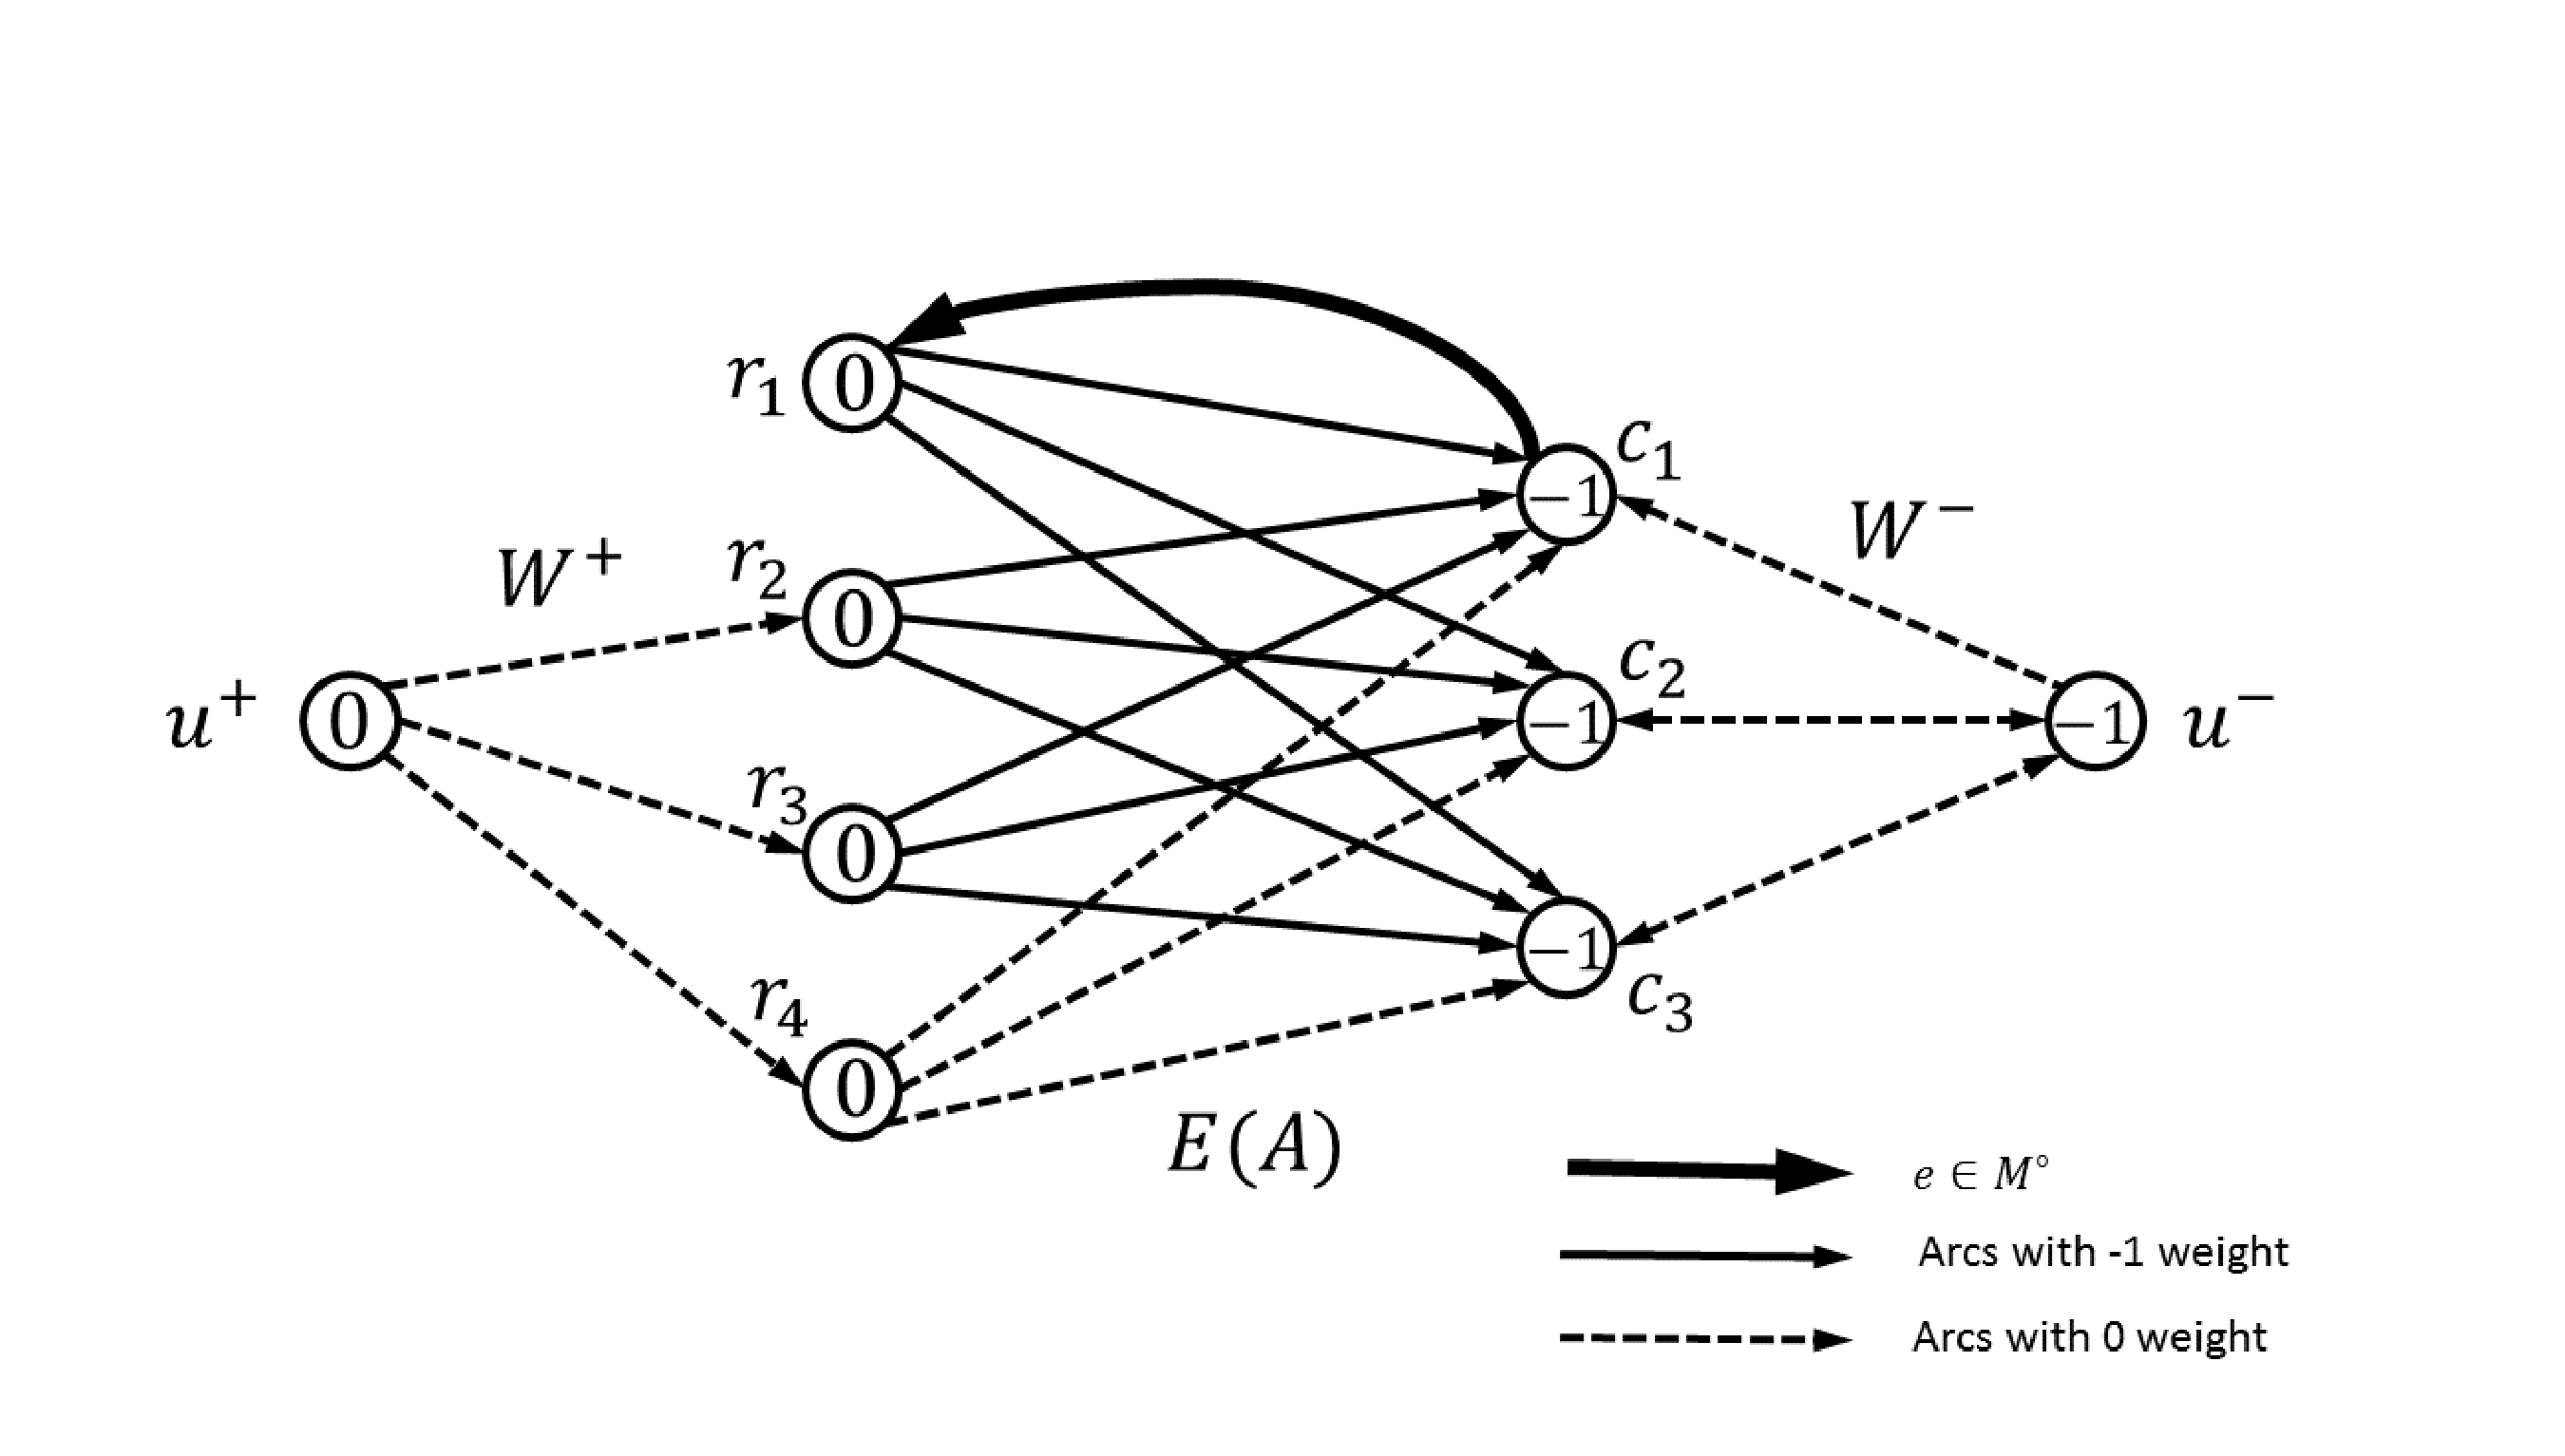
\includegraphics[width=10cm]{figauxgraph1.eps}
\caption{Auxiliary graph $ G_{M_1}$}
\label{figaux1}
\end{figure}

In $ G_{M_1} $, $ \varphi (i) $, the length of the shortest path from $ u^{+} $ to $ i \in V $, is computed as follows:
\begin{align*}
\varphi (r_1) &= \varphi (r_2) = \varphi (r_3) = \varphi (r_4) = 0,\\
\varphi (c_1) &= \varphi (c_2) = \varphi (c_3) = \varphi (u^{-}) = -1.
\end{align*}
Therefore, an optimal dual solution is 
\begin{equation}
p = \begin{pmatrix} 0 & 0 & 0 & 0 \end{pmatrix}, \quad
q = \begin{pmatrix} 0 & 0 & 0 \end{pmatrix}, \quad
t   = 1. \label{eqexdual}
\end{equation}

\paragraph{Step 2: Test for Tightness\\}
With the optimal dual solution in equation (\ref{eqexdual}), $ A^{\ast} $ is defined as follows:
\begin{equation}
A^{\ast} = \left( \begin{array}{ccccc}
1 & & 1 & & 1 \\ 1 & & 1 & & 1 \\ 1 & & 1 & & 1 \\ 0 & & 0 & & 0 
\end{array} \right).
\end{equation}
Since $ \rank A^{\ast} = 1 = k $, go to Step 3.

\paragraph{Step 3: Matrix Modification\\}
The $ 3 \times 1 $ matrix $ \tilde{U} $ satisfies following equation:
\[ \tilde{U} \cdot 1 + \begin{pmatrix} 1 \\ 1 \\ 0 \end{pmatrix} = O. \]
Therefore, $ \tilde{U} = \begin{pmatrix} -1 & -1 & 0 \end{pmatrix}^{\top} $. Then, rational matrix $ A(x) $ is modified as follows:
\begin{align*}
A'(x) &= \begin{pmatrix} A[I^{\ast}_1 , C] \\ \tilde{U} \cdot x^{p_{r_1}} \cdot A[I^{\ast}_1,C] (x) + A[R \setminus I^{\ast}_1 , C] (x)  \end{pmatrix}\\
&=  \left( \begin{array}{ccccc}
x+1 & & x+3 & & x+2 \\ 1 & & 3 & & 2 \\ 0 & & 0 & & -1 \\ 2 & & 1 & & 3 \\
\end{array} \right).
\end{align*}

Next, we implement same step (Step 1 and 2) to confirm that the modification makes sense.

\paragraph{Step 1 and 2\\}
In the same way, we can obtain the optimal dual solution:
\begin{equation}
p = \begin{pmatrix} 1 & 0 & 0 & 0 \end{pmatrix}, \quad
q = \begin{pmatrix} 0 & 0 & 0 \end{pmatrix}, \quad
t   = 0. \label{eqexdual2}
\end{equation}
Then, $ A^{\ast} $ is modified as follows:
\begin{equation}
A^{\ast} = \left( \begin{array}{ccccc}
1 & & 1 & & 1 \\ 1 & & 3 & & 2 \\ 0 & & 0 & & -1 \\ 2 & & 1 & & 3 
\end{array} \right).
\end{equation}

To compute $ \rank A^{\ast} $, we execute the Gaussian Elimination as stated in section \ref{test}:
\begin{equation}
\left( \begin{array}{ccccc}
1 & & 1 & & 1 \\ 1 & & 3 & & 2 \\ 0 & & 0 & & -1 \\ 2 & & 1 & & 3 
\end{array} \right)
\rightarrow
\left( \begin{array}{ccccc}
1 & & 1 & & 1 \\ 0 & & 2 & & 1 \\ 0 & & 0 & & -1 \\ 0 & & -1 & & 1 
\end{array} \right)
\rightarrow
\left( \begin{array}{ccccc}
1 & & 1 & & 1 \\ 0 & & 0 & & 3 \\ 0 & & 0 & & -1 \\ 0 & & -1 & & 1 
\end{array} \right)
\rightarrow
\left( \begin{array}{ccccc}
1 & & 1 & & 1 \\ 0 & & 0 & & 0 \\ 0 & & 0 & & -1 \\ 0 & & -1 & & 1 
\end{array} \right). \label{eqexge}
\end{equation}
Since $ \rank A^{\ast} = 3 $, go to Step 4.

\paragraph{Step 4: Outputs and Updates\\} 
From the equation (\ref{eqexge}), $ I^{\ast}_3 = \{ r_1 , r_3, r_4\} $ and $ J^{\ast}_3 = C $.
Solving the weighted bipartite matching problem over $ G = ( I^{\ast}_3 \cup J^{\ast}_3 , E_3 , c ) $ (Fig. \ref{figwm}) where $ E_3 \subseteq E $ is defined as $ E_3 = E(A) \cap ( I^{\ast}_3 \times J^{\ast}_3 ) $, we obtain $ M_3 = \{ (r_1,c_1), (r_3,c_3), (r_4,c_2) \} $.
As a result, $ \delta_2 (A) $ and $ \delta_3 (A) $ is calculated as follows:
\begin{align*}
\delta_2 (A) &= \delta_1 (A) + 1 \cdot 0 = 1,\\
\delta_2 (A) &= \delta_1 (A) + 2 \cdot 0 = 1.
\end{align*}
Since $ k = \rank A^{\ast} = 3 $ and $ |C| = 3 $, the algorithm has finished. 

\begin{figure}
\centering
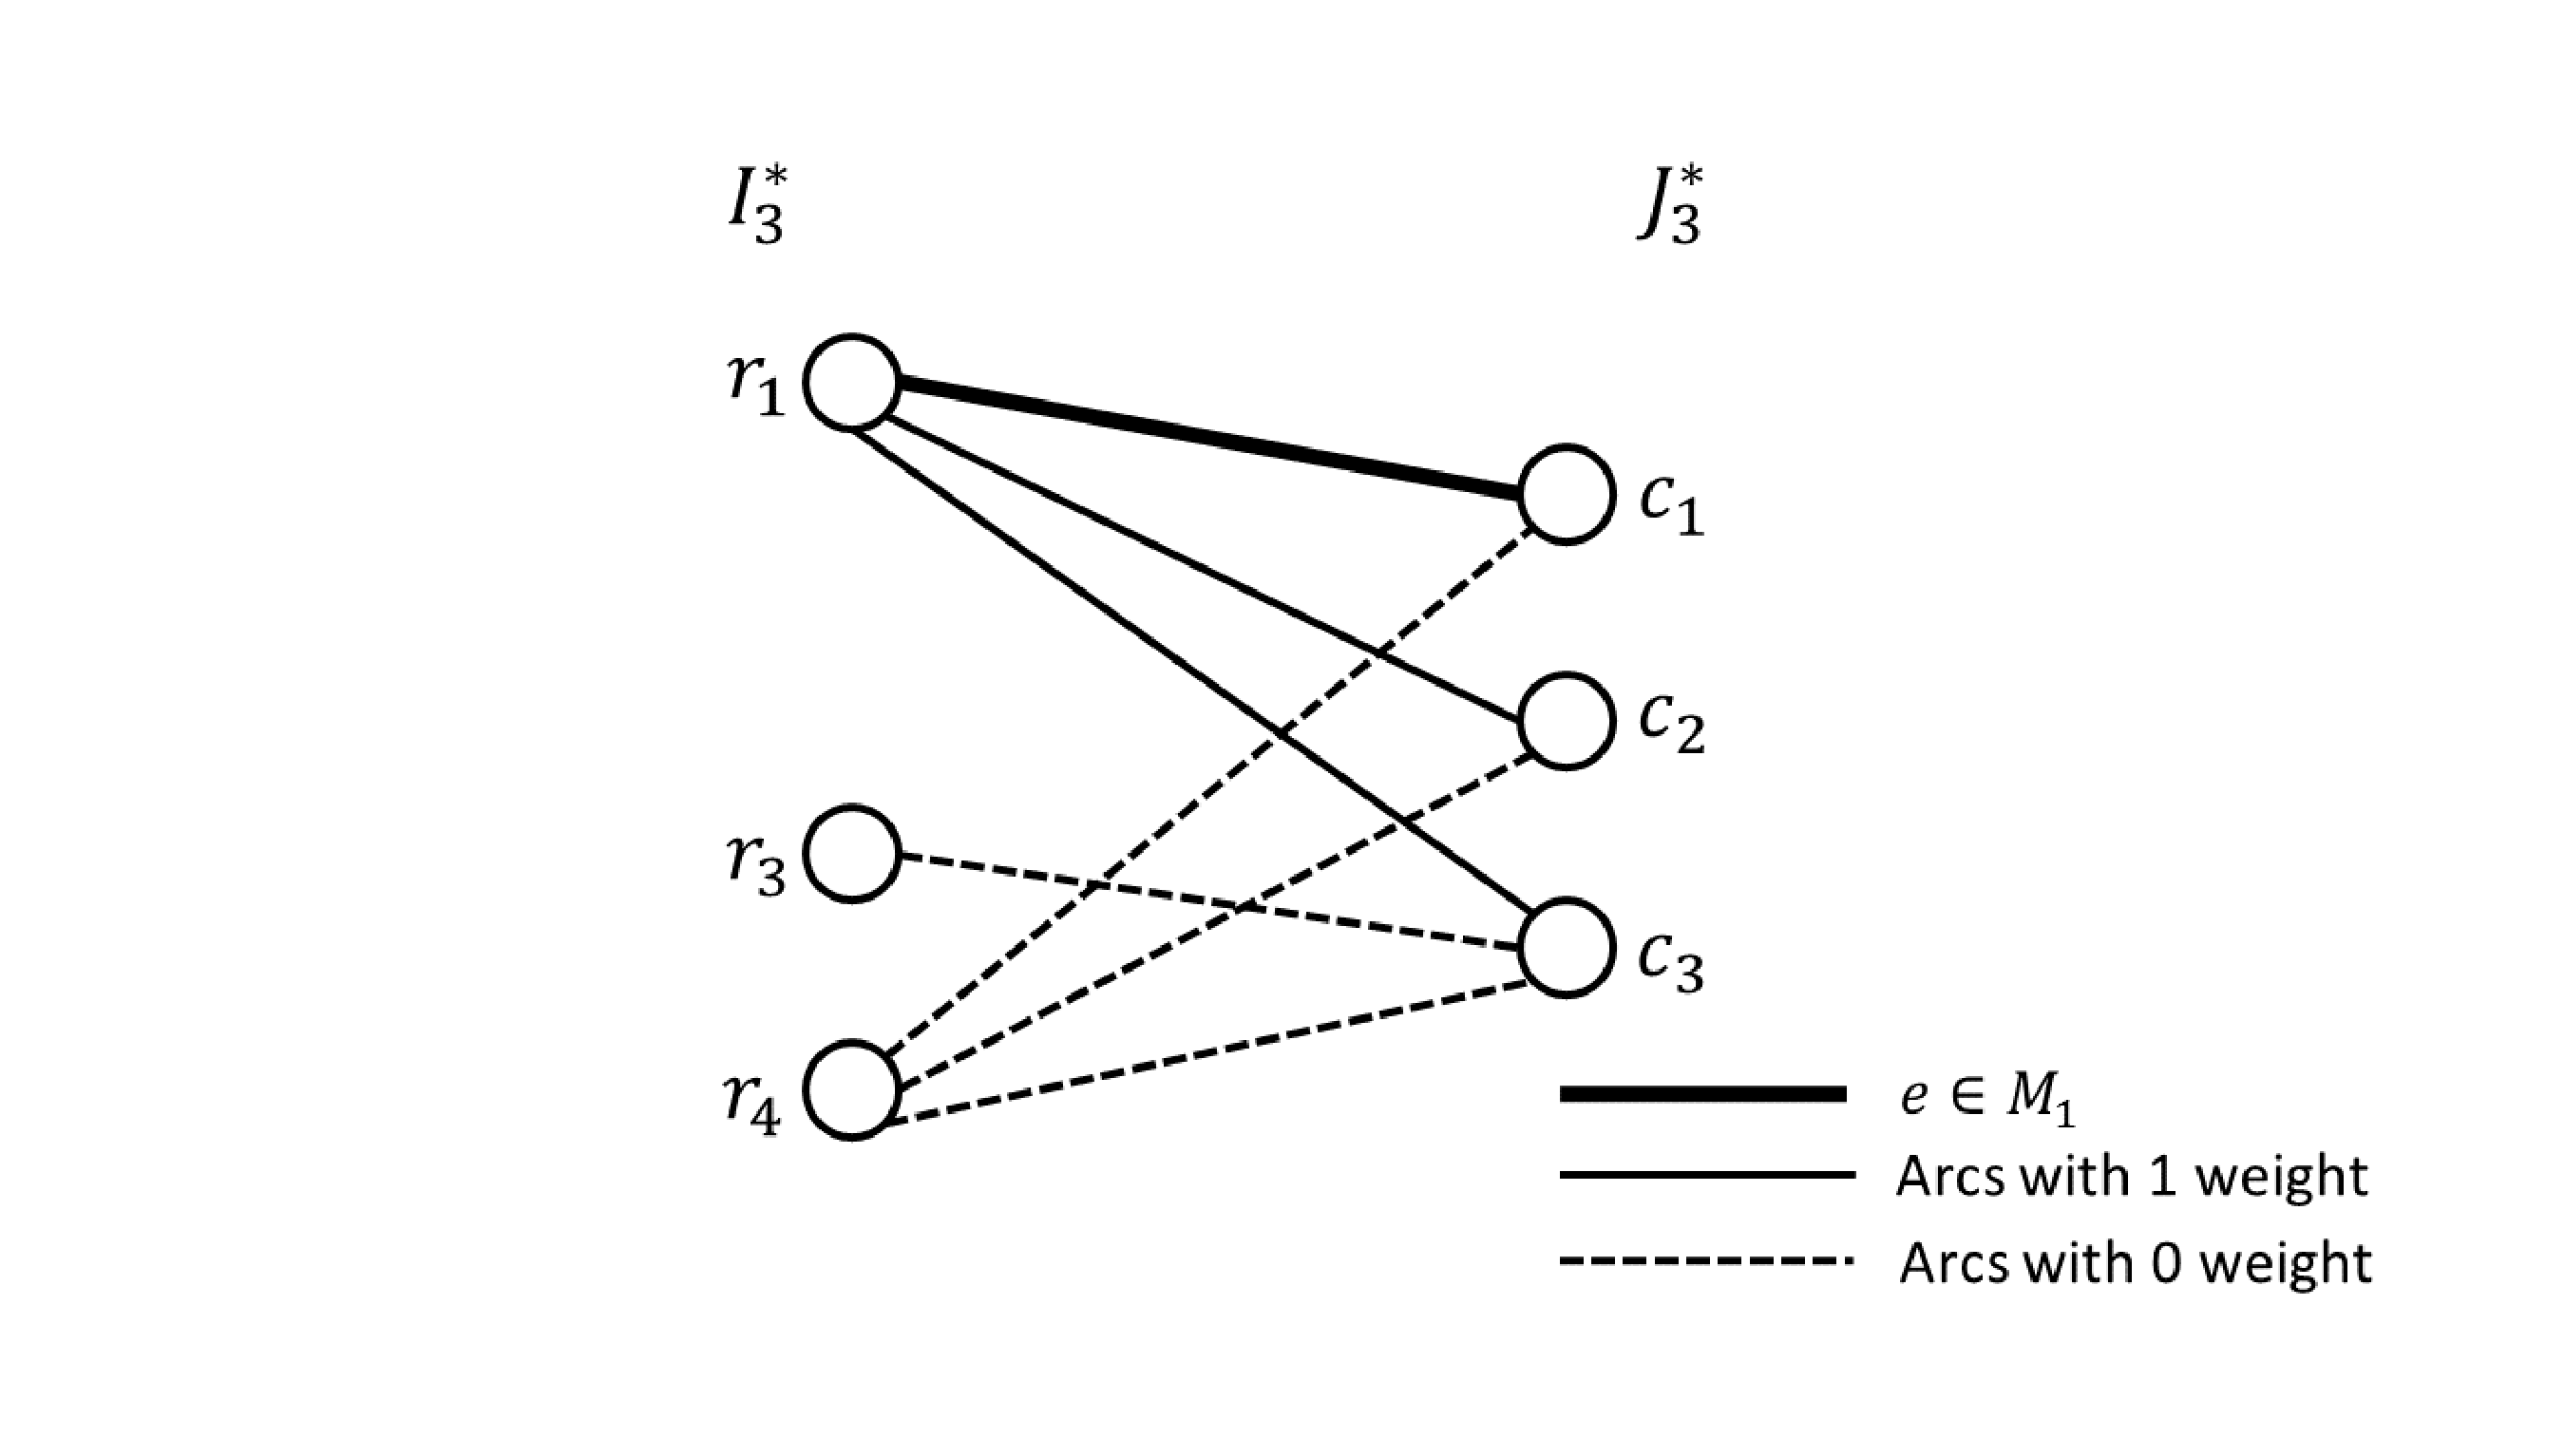
\includegraphics[width=10cm]{figexwm.eps}
\caption{$G= (I^{\ast}_3 \cup J^{\ast}_3,E_3,c)$}
\label{figwm}
\end{figure}

\end{example}


\section{Complexity Analysis}
\label{ca}
\subsection{Worst Case Analysis}
\label{wca}
Fist of all, we show the definition of parameters in Table \ref{tabp} 
and time complexity of each operation in Table \ref{tabwtc}.
Time complexity of proposed algorithm is $ O (dnr(n+dmr)) $ as Theorem \ref{thmwa}

\begin{table}
\centering
\caption{The definition of parameters}
\label{tabp}  
\begin{tabular}{lll}
\hline\noalign{\smallskip}
symbol &  & definition  \\
\noalign{\smallskip}\hline\noalign{\smallskip}
$m$ & : & The number of rows \\
$n$ & : & The number of columns \\
$r$ & : & $ \rank A $ \\
$d_{\max}$ & : & $ \max \deg A_{ij} $ \\
$d_{\min}$ & : & $ \min \mathrm{ord} A_{ij} $\\
$d$ & : & $ d_{\max} - d_{\min} $\\
\noalign{\smallskip}\hline
\end{tabular}
\end{table}

\begin{table}
\centering
\caption{Time complexity of each operation}
\label{tabwtc}  
\begin{tabular}{llll}
\hline\noalign{\smallskip}
Step &  Operation & Time Complexity & Method  \\
\noalign{\smallskip}\hline\noalign{\smallskip}
\hline Step 0 & Initialization & $ O(mn)$ & Max Search \\ 
\hline Step 1 & Optimal Dual Solution & $ O(d n^2 r) $ & Single Source Shortest Path \\ 
\hline Step 2 & Calculation of Rank & $ O(d m n r^2) $ & Gaussian Elimination \\ 
\hline Step 3 & Construction of $\tilde{U}$ & $ O (dmr^3)$ & LU Decomposition \\ 
  & Matrix Modification & $ O (d^2 mnr^2)$ & Matrix Multiplication \\ 
\hline Step 4 & Construction of $M_{r^{\ast}} $ & $ O (r^3) $ & Single Source Shortest Path \\ 
\noalign{\smallskip}\hline
\end{tabular}
\end{table}

\begin{theorem}
Let $ A(x) $ be an $ m \times n $ Laurent polynomial matrix and each parameter is defined as Table \ref{tabp}.
Then, proposed algorithm runs in $ O (dnr(n+dmr)) $ time.
\label{thmwa}
\end{theorem}

\begin{proof}
We can prove the theorem by confirming that Table \ref{tabwtc} is correct.

In Step 0, we search the maximizer of $ \deg A_{ij} $. 
Therefore, it can be done in $ O (mn) $ time.

In Step 1, we construct the optimal dual solution 
by solving the single source shortest path problem. 
Since we can reweight the arc length to non-negative, 
it can be done in square time of the number of vertices($O(n+m)$).
And Step 1 executes $ O (dr) $ times in worst case. 
Because the value of $t$ decreases at least one each time and the difference between the optimal $q$ of DLP($A,1$) and DLP($A,r$) is $ r d $ at most.
Therefore, Step 1 runs in $ O (dn^2 r) $ time.

Step 2 runs in $ O ( mnr ) \times O(dr) $ time. 
Because Gaussian elimination can be done in $ O(mnr) $ time 
and it executes $ O(dr) $ times such as Step 1.

In Step 3, We can construct $ \tilde{U} $ by LU decomposition in $O(mr^2)$ time each execution. 
Therefore, it can be done in $ O (dmr^3)$ time. 
In the phase of matrix modification, 
we execute multiplication between $ ( m - s) \times s $ polynomial matrix 
and $ s \times n $ polynomial matrix if $ k = s $ holds. 
Furthermore, we can execute multipication of polynomials with degree $d$ 
in $ O ( d \log d \log \log d ) $(Cantor--Kaltofen\cite{FMP}). 
Then, it can be done in $ O ( d^2 mnr^2 ) $ if we ignore $ O (\log d ) $. 

We solve the single source shortest path problem ($ r -1 $) times in the whole of Step 4. 
Moreover, the arc length of auxiliary graph can be reweight to non-negative.
Therefore, Step 4 runs in $ O(r^3)$. \qed
\end{proof}


\begin{comment}
\section{Application to Maxumum Weight $k$-Matching in Bipartite Graph}
\label{app}

Let $ G = ( U \cup V ,E , c) $ be a weighted bipartite graph with disjoint finite set $U,$ $V$, arc set $ E \subseteq U \times V $ and arc lengh $ c: E \to \mathbb{Z} $. 
\end{comment}

\section{Conclusion}
\label{conc}

The proposed algorithm runs in $ O( nr ( n + mr)) $ if we assume $ d $ is constant. 
It is more efficient than previous algorithm(Iwata--Murota--Sakuto\cite{PDCRA}) runs in $ O (mn^2r) $.



\begin{acknowledgements}
\postpone
\end{acknowledgements}


% % % % % % % % % % % % % % % % % % % %  bibliography % % % % % % % % % % % % % % % % % % % % % % % %
\begin{thebibliography}{99}
\bibitem{FMP} Cantor, D. G., Kaltofen, E.: On fast multiplication of polynomials over arbitrary algebras. Acta Informatica. {\bf 28}, 693--701 (1991)
\bibitem{SMF} Commault, C., Dion, J.M.: Structure at infinity of linear multivariable systems: A geometric approach. IEEE Trans. Automat. Control. {\bf AC-27}, 693--696 (1982)
\bibitem{AI} Cormen, T. H., Leiserson, C. E., Rivest, R. L., Stein, C.: Introduction to Algorithms. The MIT Press. Cambridge, second edition (2001)
\bibitem{VM1} Dress, A. W. M., Wenzel, W.: Valuated matroid: A new look at the greedy algorithm. Appl. Math. Lett. {\bf 3}(2), 33--35 (1990)
\bibitem{VM2} Dress, A. W. M., Wenzel, W.: Valuated matroids. Adv. Math. {\bf 93}, 214--250 (1992)
\bibitem{TI} Edmonds, J., Karp, R. M.: Theoretical improvements in algorithmic efficiency for network flow problems. Journal of ACM. {\bf 19}, 248--264 (1972)
\bibitem{DAE} Gear, C. W.: Differential algebraic equations, indeces, and integral algebraic equations. SIAM J. Number. Anal. {\bf 27}, 1527--1534 (1990)
\bibitem{PDCRA} Iwata, S., Murota, K., Sakuta, I.: Primal-dual combinatorial relaxation algorithm for the maximum degree of subdeterminants. SIAM J. Sci. Comput. {\bf 17}, 993--1012 (1996)
\bibitem{MP} Iwata, S., Takamatsu, M.: Computing the maximum degree of minors in mixed polynomial matrices via combinatorial relaxation. Algorithmica {\bf 66}, 346--368 (2013)
\bibitem{HM} Kuhn, H.: The hungarian method for the assignment problem. Naval Research Logistics Quarterly {\bf 2}, 83--97 (1955)
\bibitem{SC} Lin, C. T.: Structural controllability. IEEE Trans. Automat. Control {\bf AC-19}, 201--208 (1974)
\bibitem{CRA} Murota, K.: Computing Puiseux-series solutions to determinantal equations via combinatorial relaxation. SIAM J. Comput. {\bf 19}, 1132--1161 (1990)
\bibitem{PCRA} Murota, K.: Combinatorial relaxation algorithm for the maximum degree of subdeterminants: Computing Smith--Mcmillan form at infinity and structural indices in Kronecker form. Appl. Algebra Eng. Commun. Comput. {\bf 6}, 251--273 (1995)
\bibitem{DCRA} Murota, K.: Computing the degree of determinants via combinatorial relaxation. SIAM J. Comput. {\bf 24}, 765--796 (1995)
\bibitem{VB} Murota, K.: Finding optimal minors of valuated bimatroids. Appl. Math. Lett. {\bf 8}, 37--42 (1995)
\bibitem{MMSA} Murota, K.: Matrices and Matroids for Systems Analysis. Springer, Berlin (2000)
\bibitem{TNP} Tomizawa, N.: On some techniques useful for solution of transportation network problems. Networks {\bf 1}, 173--194 (1971)
\bibitem{RMS} Verghese, G.C., Kailath, T.: Rational matrix structure. IEEE Trans. Autom. Control {\bf AC-26}, 443--439 (1981)
\end{thebibliography}
\end{document}